\documentclass[12pt,a4paper]{report}
\usepackage[utf8]{inputenc}
\usepackage{amsmath}
\usepackage{amsfonts}
\usepackage{amssymb}
\usepackage{bm}
\usepackage{graphicx}
\usepackage{listings}
\usepackage[colorlinks = true,
            linkcolor = black,
            urlcolor  = black,
            citecolor = blue,
            anchorcolor = black]{hyperref}
\graphicspath{ {./pics/} } %set path to folder with images

\usepackage{nccmath}
\newenvironment{mpmatrix}{\begin{medsize}\begin{pmatrix}}%
{\end{pmatrix}\end{medsize}}%

\usepackage{booktabs, rotating}
\usepackage[verbose]{placeins}

\usepackage{natbib}
\bibliographystyle{plainnat}

\DeclareMathOperator*{\argmin}{\arg\!\min}

%\begin{figure}[h!]
%\begin{minipage}[h!]{0.49\textwidth}
%	\center{\includegraphics[width=0.8 \linewidth]{cgrid.png}}
%  	\caption{Computational conventional Cartesian grid. Elastic constants and density are given for each point separately, $U_i$ denotes to  displacement wavefield component corresponding to the node}
%  	\label{fig:comp_grid_param}
%\end{minipage}
%\hfill
%\begin{minipage}[h!]{0.49\textwidth}
%	\center{\includegraphics[width=0.8 \linewidth]{2D_stencil.png}}
%  	\caption{Nine-point stencil used for computation of spatial derivatives}
%  	\label{fig:2D_wg_stencil}
%\end{minipage}
%\end{figure}

\title{AMCS 312. Course project}
\author{Oleg Ovcharenko}
\begin{document}
\maketitle

\section*{Abstract}
In this project we explore scalability of a hyperbolic problem solved in finite-difference approximation with implicit time stepping using Krylov methods implemented in PETSc.

\section*{Introduction}

There is a variety of computational methods such as Finite-Element Method (FEM) \citep{strang1973analysis}, spectral-element method(SEM) \citep{komatitsch1999introduction} and others, but the most popular one is Finite-difference method(FDM) that is widely used due to it's simplicity, speed, relative easiness in implementation and parallelization.

We won't get into details of finite-difference theory, but one could find sufficient introduction in \cite{moczo2007finite}. The general idea is simple -- solve equation in FD approximation where all spatial and temporal derivatives are replaced with their descritized on grid analogous. There are two principal points to choose: how to discretize derivatives in space and how to discretize them in time. As an example, this choice leads to such methods as pseud-spectral methods(PSM) \citep{kosloff1982forward}, where time derivatives could be approximated in variety of ways, but spatial derivatives are computed using Fourier transforms. Also there is a choice of grid types with their pros and cons, for example: conventional collocated grid, staggered grid \cite{Virieux1984, Virieux1986}, rotated staggered grid \citep{saenger2000modeling} and others. The way of approximation of time derivatives defines two basic time stepping methods: explicit and implicit. Explicit methods calculate the state of a system at a later time from the state of the system at the current time, while implicit methods find a solution by solving an equation involving both the current state of the system and the later one. Implicit methods require an extra computation and it can be much harder to implement them. Despite these difficulties, implicit methods are used because there are many problems arising in practice for which the use of an explicit method requires impractically small time steps $\Delta t$ to keep the error in the result bounded (to satisfy Courant-Friedrichs-Lewy condition \citep{courant1928partiellen}). For such problems, to achieve given accuracy, it takes much less computational time to use an implicit method with larger time steps, even taking into account that one needs to solve the whole system of equations at each time step. So it depends upon the problem to be solved, whether one should use an explicit or implicit method.\\

\section*{Motivation}
Whe have chosen seismic wave propagation as the problem of interest as this topic has always been an area of interest among Earth science researchers because wave propagation is widely used both in exploration and global geophysics. On exploration scale seismic waves are propagated at each step of full-waveform inversion and on global scale this is done for modeling of surface waves, to model earthquake responses and etc. Implicit time stepping methods are very promising, but their behavior on large scales is not explored well yet.


\section*{Approach}
Implicit FD operators have been relatively recently introduced to solve seismic wave propagation problems \citep{liu2009practical, kosloff2010acoustic, chu2010frequency}, but one could already note their potential driven also by steady growth of HPC facilities. That is why we have chosen implicit time stepping in order to check scalability and overall performance of this approach as currently the majority of wave propagators are implemented with explicit schemes. In general, use of implicit method was motivated by several factors. First, we were impressed by performance of iterative Krylov-based methods implemented in PETSc (Portable, Extensible Toolkit for Scientific Computation) for solving systems of linear and non-linear equations. Second, it is said, that using implicit method one could choose larger time step and fewer grid points per wavelength, whereas in explicit methods one has to satisfy CFL condition and thus use very small time step for fine grids. Third, \citep{chu2012implicit, chu2010frequency}  showed that using implicit numerical operators higher accuracy might be achieved with negligible additional costs.\\

\section*{Framework}
We consider acoustic wave propagation due to it's simplicity and as it is sufficient for the purpuses of the study. Mathematically acoustic wave propagation in homogeneous media can be expressed as a second-order hyperbolic PDE given as eq.~\ref{eq:ac}. Chosing the grid type and spatial derivative discretization for this equation, we follow reasoning of \cite{geller2005comparison} who showed that “Displacement only” schemes on collocated grids can be equivalent or in some cases more efficient in terms of cost then widely used "Velocity-stress" schemes on staggered grid. Spatial derivative's approximations are chosen to be based on Taylor series expansion as this formulation fits well our needs. To sum up:
\begin{enumerate}
\item[] \textbf{Equation:} Strong form of equation of motion in displacement formulation
\item[] \textbf{Discretization:} Finite differences in time domain (FDTD)
\item[] \textbf{Time stepping:} Implicit
\item[] \textbf{Accuracy:} $O\left(2,4\right)$
\item[] \textbf{Domain:} 3D homogeneous isotropic media with constant velocity
\item[] \textbf{Programming:} C/C++ with PETSc 3.6.1\\
\end{enumerate} 

\subsection*{3D acoustic wave equation}
Strong form of acoustic wave equation for homogeneous media in displacement formulation could be expressed as follows
\begin{equation}
\frac{\partial^2 u}{\partial t^2} - c^2 \left(\frac{\partial^2 u}{\partial x^2} + \frac{\partial^2 u}{\partial y^2} + \frac{\partial^2 u}{\partial z^2}\right) = f
\label{eq:ac}
\end{equation}

We discretize it with 2nd order of accuracy both in space and time, $O\left(2,2\right)$. Implicit time stepping requires backward time derivative approximation, whereas spacial derivatives are approximated with centered scheme.

\begin{equation}
\begin{aligned}
&\frac{2 U^{n+1}_{i,j,k} - 5 U^{n}_{i,j,k} + 4 U^{n-1}_{i,j,k} - U^{n-2}_{i,j,k}}{\Delta t^2} = \\
& c^2_{i,j,k} \frac{U^{n+1}_{i+1,j,k} - 2 U^{n+1}_{i,j,k} + U^{n+1}_{i-1,j,k}}{\Delta x^2} +\\
& c^2_{i,j,k} \frac{U^{n+1}_{i,j+1,k} - 2 U^{n+1}_{i,j,k} + U^{n+1}_{i,j-1,k}}{\Delta y^2} + \\
& c^2_{i,j,k} \frac{U^{n+1}_{i,j,k+1} - 2 U^{n+1}_{i,j,k} + U^{n+1}_{i,j,k-1}}{\Delta z^2} + f_{i,j,k}
\end{aligned}
\end{equation}

Hence,
\if0
\begin{equation}
\begin{aligned}
2 U^{n+1}_{i,j,k} - 5 U^{n}_{i,j,k} + 4 U^{n-1}_{i,j,k} - U^{n-2}_{i,j,k} = c^2_{i,j,k} \Delta t^2 (\\
& \frac{U^{n+1}_{i+1,j,k} - 2 U^{n+1}_{i,j,k} + U^{n+1}_{i-1,j,k}}{\Delta x^2} +\\
& \frac{U^{n+1}_{i,j+1,k} - 2 U^{n+1}_{i,j,k} + U^{n+1}_{i,j-1,k}}{\Delta y^2} + \\
& \frac{U^{n+1}_{i,j,k+1} - 2 U^{n+1}_{i,j,k} + U^{n+1}_{i,j,k-1}}{\Delta z^2} )
\end{aligned}
\end{equation}

\begin{equation}
\begin{aligned}
2 U^{n+1}_{i,j,k} - c^2_{i,j,k} \Delta t^2 (
\frac{U^{n+1}_{i+1,j,k} - 2 U^{n+1}_{i,j,k} + U^{n+1}_{i-1,j,k}}{\Delta x^2} +
\frac{U^{n+1}_{i,j+1,k} - 2 U^{n+1}_{i,j,k} + U^{n+1}_{i,j-1,k}}{\Delta y^2} + \\
\frac{U^{n+1}_{i,j,k+1} - 2 U^{n+1}_{i,j,k} + U^{n+1}_{i,j,k-1}}{\Delta z^2} ) \\= \\ 5 U^{n}_{i,j,k} - 4 U^{n-1}_{i,j,k} + U^{n-2}_{i,j,k} + f_{i,j,k}
\end{aligned}
\end{equation}
\fi

\begin{equation}
\begin{aligned}
& U^{n+1}_{i,j,k} \left(2 \Delta x \Delta y \Delta z + 2 c^2_{i,j,k} \Delta t^2 \left( \frac{\Delta y \Delta z}{\Delta x} + \frac{\Delta x \Delta z}{\Delta y}+ \frac{\Delta x \Delta y}{\Delta z}\right)\right) + \\
& U^{n+1}_{i+1,j,k}  \left( -c^2_{i+1,j,k} \Delta t^2\ \frac{\Delta y \Delta z}{\Delta x}\right) + \\
& U^{n+1}_{i-1,j,k}  \left( -c^2_{i-1,j,k} \Delta t^2\ \frac{\Delta y \Delta z}{\Delta x}\right) + \\
& U^{n+1}_{i,j+1,k}  \left( -c^2_{i,j+1,k} \Delta t^2\ \frac{\Delta x \Delta z}{\Delta y}\right) + \\
& U^{n+1}_{i,j-1,k}  \left( -c^2_{i,j-1,k} \Delta t^2\ \frac{\Delta x \Delta z}{\Delta y}\right) + \\
& U^{n+1}_{i,j,k+1}  \left( -c^2_{i,j,k+1} \Delta t^2\ \frac{\Delta x \Delta y}{\Delta z}\right) + \\
& U^{n+1}_{i,j,k-1}  \left( -c^2_{i,j,k-1} \Delta t^2\ \frac{\Delta x \Delta y}{\Delta z}\right) = \\
& \Delta x \Delta y \Delta z \left( 5 U^{n}_{i,j,k} - 4 U^{n-1}_{i,j,k} + U^{n-2}_{i,j,k} + \Delta t^2 f_{i,j,k} \right)
\end{aligned}
\label{eq:22}
\end{equation}

At each time step we will solve system
\begin{equation}
Ax=b
\end{equation}
where lhs. will consist of values from lhs. of eq.~\ref{eq:22} rhs. will be rhs. of the same equation. As one could notice, matrix $A$ is a 7 diagonal matrix (Fig.~\ref{fig:m22}) that has to be inverted a teach time step in implicit methods. It worth noticing again that we are not going to invert this matrix directly, but do it using iterative Krylov methods that find $A^{-1} b$ approximation cheaper in terms of memory and which are well parallelizable.\\

Now let us do the same but for $O\left(2,4\right)$, and get as a result 13 diagonal matrix (Fig.~\ref{fig:m24}).
\begin{equation}
\begin{aligned}
&\frac{2 U^{n+1}_{i,j,k} - 5 U^{n}_{i,j,k} + 4 U^{n-1}_{i,j,k} - U^{n-2}_{i,j,k}}{\Delta t^2} = \\
& c^2_{i,j,k} \frac{-U^{n+1}_{i+2,j,k} + 16 U^{n+1}_{i+1,j,k} - 30 U^{n+1}_{i,j,k} + 16 U^{n+1}_{i-1,j,k} - U^{n+1}_{i-2,j,k}}{12\Delta x^2} +\\
& c^2_{i,j,k} \frac{-U^{n+1}_{i,j+2,k} + 16 U^{n+1}_{i,j+2,k} - 30 U^{n+1}_{i,j,k} + 16 U^{n+1}_{i,j-1,k} - U^{n+1}_{i,j-2,k}}{12\Delta y^2} +\\
& c^2_{i,j,k} \frac{-U^{n+1}_{i,j,k+2} + 16 U^{n+1}_{i,j,k+1} - 30 U^{n+1}_{i,j,k} + 16 U^{n+1}_{i,j,k-1} - U^{n+1}_{i,j,k-2}}{12\Delta z^2} +\\
\end{aligned}
\end{equation}

\begin{equation}
\begin{aligned}
& U^{n+1}_{i,j,k} \left(2 \Delta x \Delta y \Delta z + 30\ c^2_{i,j,k} \Delta t^2 \left( \frac{\Delta y \Delta z}{12 \Delta x} + \frac{\Delta x \Delta z}{12 \Delta y}+ \frac{\Delta x \Delta y}{12 \Delta z}\right)\right) + \\
& U^{n+1}_{i+2,j,k}  \left(c^2_{i+2,j,k} \Delta t^2\ \frac{\Delta y \Delta z}{12 \Delta x}\right) + \\
& U^{n+1}_{i+1,j,k}  \left( -16\ c^2_{i+1,j,k} \Delta t^2\ \frac{\Delta y \Delta z}{12 \Delta x}\right) + \\
& U^{n+1}_{i-1,j,k}  \left( -16\ c^2_{i-1,j,k} \Delta t^2\ \frac{\Delta y \Delta z}{12 \Delta x}\right) + \\
& U^{n+1}_{i-2,j,k}  \left(c^2_{i-2,j,k} \Delta t^2\ \frac{\Delta y \Delta z}{12 \Delta x}\right) + \\
& U^{n+1}_{i,j+2,k}  \left(c^2_{i,j+2,k} \Delta t^2\ \frac{\Delta x \Delta z}{12 \Delta y}\right) + \\
& U^{n+1}_{i,j+1,k}  \left( -16\ c^2_{i,j+1,k} \Delta t^2\ \frac{\Delta x \Delta z}{12 \Delta y}\right) + \\
& U^{n+1}_{i,j-1,k}  \left( -16\ c^2_{i,j-1,k} \Delta t^2\ \frac{\Delta x \Delta z}{12 \Delta y}\right) + \\
& U^{n+1}_{i,j-2,k}  \left(c^2_{i,j-2,k} \Delta t^2\ \frac{\Delta x \Delta z}{12 \Delta y}\right) + \\
& U^{n+1}_{i,j,k+2}  \left(c^2_{i,j,k+2} \Delta t^2\ \frac{\Delta x \Delta y}{12 \Delta z}\right) + \\
& U^{n+1}_{i,j,k+1}  \left( -16\ c^2_{i,j,k+1} \Delta t^2\ \frac{\Delta x \Delta y}{12 \Delta z}\right) + \\
& U^{n+1}_{i,j,k-1}  \left( -16\ c^2_{i,j,k-1} \Delta t^2\ \frac{\Delta x \Delta y}{12 \Delta z}\right) + \\
& U^{n+1}_{i,j,k-2}  \left(c^2_{i,j,k-2} \Delta t^2\ \frac{\Delta x \Delta y}{12 \Delta z}\right) = \\
& \Delta x \Delta y \Delta z \left( 5 U^{n}_{i,j,k} - 4 U^{n-1}_{i,j,k} + U^{n-2}_{i,j,k} + \Delta t^2 f_{i,j,k} \right)
\end{aligned}
\end{equation}

In case of homogeneous isotropic media, matrix $A$ will be symmetric and positive definite, hence the most convenient choice of solver is CG with Schwarz preconditionner and ilu as sub-preconditionner. After simple test Schwarz levels of overlap we found that the best performance was reached when it was 2.

\begin{figure}[h!]
\begin{minipage}[h!]{0.49\textwidth}
	\center{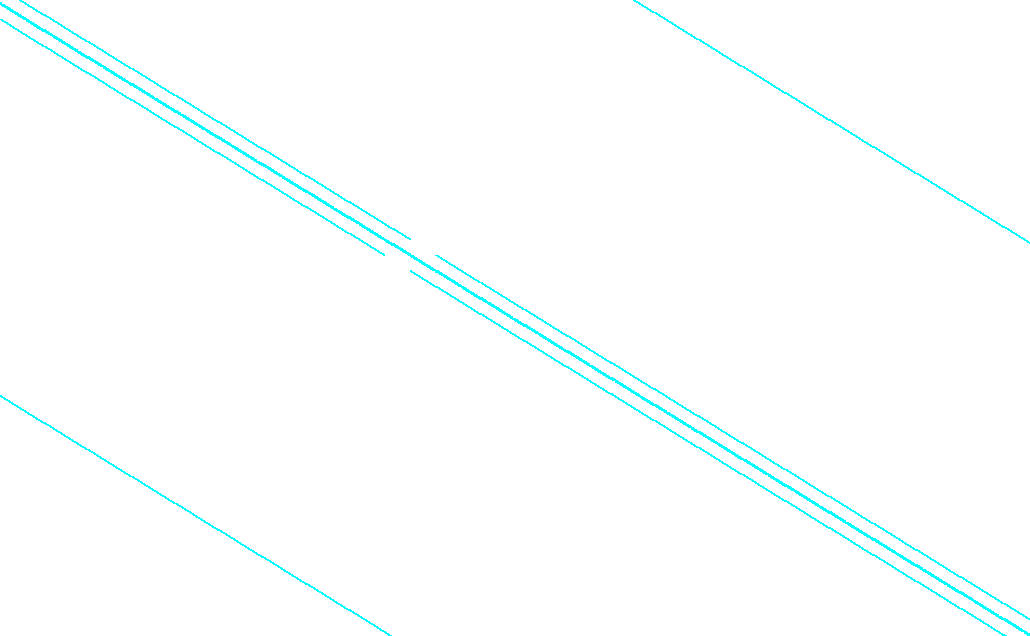
\includegraphics[width=0.9 \linewidth]{7b.png}}
  	\caption{Zoomed 7 diagonal matrix for $O(2,2)$}
  	\label{fig:m22}
\end{minipage}
\hfill
\begin{minipage}[h!]{0.49\textwidth}
	\center{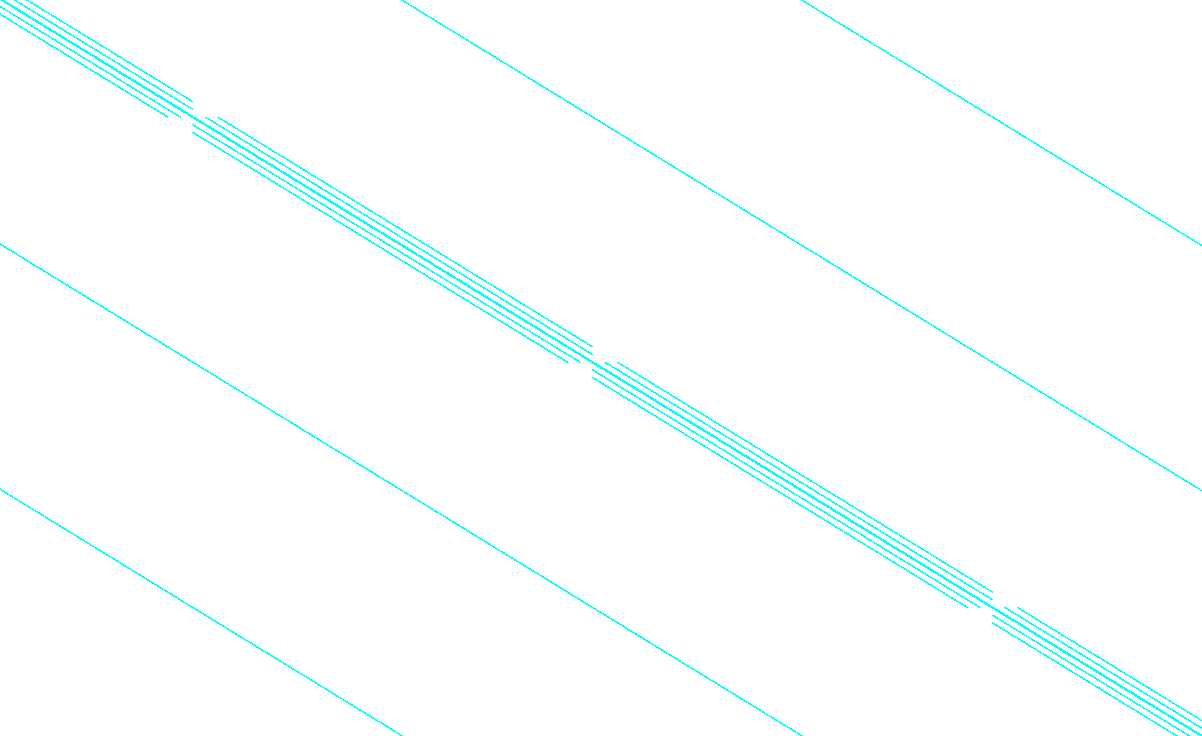
\includegraphics[width=0.9 \linewidth]{13b.png}}
  	\caption{Zoomed 13 diagonal matrix for $O(2,4)$}
  	\label{fig:m24}
\end{minipage}
\end{figure}

\section*{Results and Significance}

\section*{Lessons Learned and Future Work}

\bibliography{biblioo}
\end{document}
